\documentclass[11pt]{article}

\newcommand{\yourname}{Kevin Zhang}

\def\comments{0}

%format and packages

%\usepackage{algorithm, algorithmic}
\usepackage{tikz}
\usepackage{algpseudocode}
\usepackage{amsmath, amssymb, amsthm}
\usepackage{tcolorbox}
\usepackage{enumerate}
\usepackage{enumitem}
\usepackage{framed}
\usepackage{verbatim}
\usepackage[margin=1.0in]{geometry}
\usepackage{microtype}
\usepackage{kpfonts}
\usepackage{palatino}
	\DeclareMathAlphabet{\mathtt}{OT1}{cmtt}{m}{n}
	\SetMathAlphabet{\mathtt}{bold}{OT1}{cmtt}{bx}{n}
	\DeclareMathAlphabet{\mathsf}{OT1}{cmss}{m}{n}
	\SetMathAlphabet{\mathsf}{bold}{OT1}{cmss}{bx}{n}
	\renewcommand*\ttdefault{cmtt}
	\renewcommand*\sfdefault{cmss}
	\renewcommand{\baselinestretch}{1.06}

\usepackage[boxruled,vlined,nofillcomment]{algorithm2e}
	\SetKwProg{Fn}{Function}{\string:}{}
	\SetKwFor{While}{While}{}{}
	\SetKwFor{For}{For}{}{}
	\SetKwIF{If}{ElseIf}{Else}{If}{:}{ElseIf}{Else}{:}
	\SetKw{Return}{Return}
	

%enclosure macros
\newcommand{\paren}[1]{\ensuremath{\left( {#1} \right)}}
\newcommand{\bracket}[1]{\ensuremath{\left\{ {#1} \right\}}}
\renewcommand{\sb}[1]{\ensuremath{\left[ {#1} \right\]}}
\newcommand{\ab}[1]{\ensuremath{\left\langle {#1} \right\rangle}}

%probability macros
\newcommand{\ex}[2]{{\ifx&#1& \mathbb{E} \else \underset{#1}{\mathbb{E}} \fi \left[#2\right]}}
\newcommand{\pr}[2]{{\ifx&#1& \mathbb{P} \else \underset{#1}{\mathbb{P}} \fi \left[#2\right]}}
\newcommand{\var}[2]{{\ifx&#1& \mathrm{Var} \else \underset{#1}{\mathrm{Var}} \fi \left[#2\right]}}

%useful CS macros
\newcommand{\poly}{\mathrm{poly}}
\newcommand{\polylog}{\mathrm{polylog}}
\newcommand{\zo}{\{0,1\}}
\newcommand{\pmo}{\{\pm1\}}
\newcommand{\getsr}{\gets_{\mbox{\tiny R}}}
\newcommand{\card}[1]{\left| #1 \right|}
\newcommand{\set}[1]{\left\{#1\right\}}
\newcommand{\negl}{\mathrm{negl}}
\newcommand{\eps}{\varepsilon}
\DeclareMathOperator*{\argmin}{arg\,min}
\DeclareMathOperator*{\argmax}{arg\,max}
\newcommand{\eqand}{\qquad \textrm{and} \qquad}
\newcommand{\ind}[1]{\mathbb{I}\{#1\}}
\newcommand{\sslash}{\ensuremath{\mathbin{/\mkern-3mu/}}}
\newcommand{\pipe}{\hspace{3pt}|\hspace{3pt}}

%mathbb
\newcommand{\N}{\mathbb{N}}
\newcommand{\R}{\mathbb{R}}
\newcommand{\Z}{\mathbb{Z}}
%mathcal
\newcommand{\cA}{\mathcal{A}}
\newcommand{\cB}{\mathcal{B}}
\newcommand{\cC}{\mathcal{C}}
\newcommand{\cD}{\mathcal{D}}
\newcommand{\cE}{\mathcal{E}}
\newcommand{\cF}{\mathcal{F}}
\newcommand{\cL}{\mathcal{L}}
\newcommand{\cM}{\mathcal{M}}
\newcommand{\cO}{\mathcal{O}}
\newcommand{\cP}{\mathcal{P}}
\newcommand{\cQ}{\mathcal{Q}}
\newcommand{\cR}{\mathcal{R}}
\newcommand{\cS}{\mathcal{S}}
\newcommand{\cU}{\mathcal{U}}
\newcommand{\cV}{\mathcal{V}}
\newcommand{\cW}{\mathcal{W}}
\newcommand{\cX}{\mathcal{X}}
\newcommand{\cY}{\mathcal{Y}}
\newcommand{\cZ}{\mathcal{Z}}

%theorem macros
\newtheorem{thm}{Theorem}
\newtheorem{lem}[thm]{Lemma}
\newtheorem{fact}[thm]{Fact}
\newtheorem{clm}[thm]{Claim}
\newtheorem{rem}[thm]{Remark}
\newtheorem{coro}[thm]{Corollary}
\newtheorem{prop}[thm]{Proposition}
\newtheorem{conj}[thm]{Conjecture}

\theoremstyle{definition}
\newtheorem{defn}[thm]{Definition}
\newtheoremstyle{case}{}{}{}{}{}{:}{ }{}
\theoremstyle{case}
\newtheorem{case}{Case}

\theoremstyle{theorem}
\newtheorem{prob}{Problem}
\newtheorem{sol}{Solution}

\tikzset{every picture/.style={line width=0.75pt}} %set default line width to 0.75pt        

\begin{document}
{\large
\noindent Name: \yourname}

\vspace{15pt}

\tikzset{every picture/.style={line width=0.75pt}} %set default line width to 0.75pt        

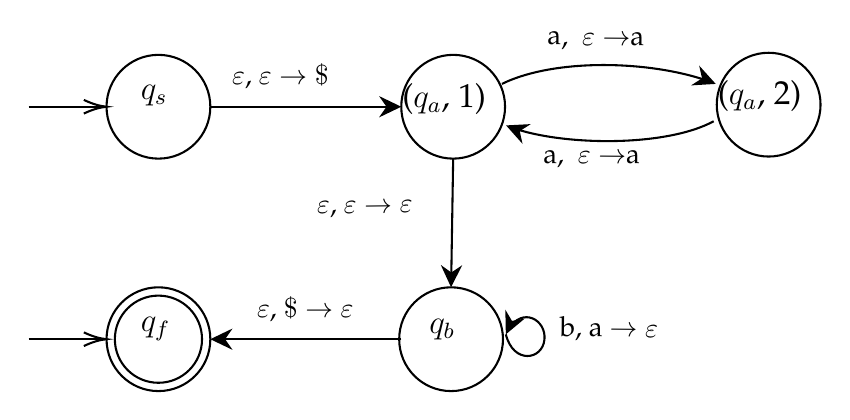
\begin{tikzpicture}[x=0.75pt,y=0.75pt,yscale=-1,xscale=1]
%uncomment if require: \path (0,195); %set diagram left start at 0, and has height of 195

%Shape: Circle [id:dp7426794074341168] 
\draw   (55,41) .. controls (55,27.19) and (66.19,16) .. (80,16) .. controls (93.81,16) and (105,27.19) .. (105,41) .. controls (105,54.81) and (93.81,66) .. (80,66) .. controls (66.19,66) and (55,54.81) .. (55,41) -- cycle ;
%Shape: Circle [id:dp5134913920036381] 
\draw   (197,41) .. controls (197,27.19) and (208.19,16) .. (222,16) .. controls (235.81,16) and (247,27.19) .. (247,41) .. controls (247,54.81) and (235.81,66) .. (222,66) .. controls (208.19,66) and (197,54.81) .. (197,41) -- cycle ;
%Straight Lines [id:da7528778304850927] 
\draw    (17.5,41) -- (53,41) ;
\draw [shift={(55,41)}, rotate = 180] [color={rgb, 255:red, 0; green, 0; blue, 0 }  ][line width=0.75]    (10.93,-3.29) .. controls (6.95,-1.4) and (3.31,-0.3) .. (0,0) .. controls (3.31,0.3) and (6.95,1.4) .. (10.93,3.29)   ;
%Straight Lines [id:da5982144898371642] 
\draw    (105,41) -- (194,41) ;
\draw [shift={(197,41)}, rotate = 180] [fill={rgb, 255:red, 0; green, 0; blue, 0 }  ][line width=0.08]  [draw opacity=0] (10.72,-5.15) -- (0,0) -- (10.72,5.15) -- (7.12,0) -- cycle    ;
%Shape: Circle [id:dp7675560256005667] 
\draw   (196,153) .. controls (196,139.19) and (207.19,128) .. (221,128) .. controls (234.81,128) and (246,139.19) .. (246,153) .. controls (246,166.81) and (234.81,178) .. (221,178) .. controls (207.19,178) and (196,166.81) .. (196,153) -- cycle ;
%Straight Lines [id:da8113476277012659] 
\draw    (222,66) -- (221.05,125) ;
\draw [shift={(221,128)}, rotate = 270.92] [fill={rgb, 255:red, 0; green, 0; blue, 0 }  ][line width=0.08]  [draw opacity=0] (10.72,-5.15) -- (0,0) -- (10.72,5.15) -- (7.12,0) -- cycle    ;
%Curve Lines [id:da1765096010716627] 
\draw    (247.38,150.66) .. controls (250.98,165.16) and (264.98,163.16) .. (265.98,153.16) .. controls (266.91,143.81) and (255.61,137.08) .. (248.74,148.1) ;
\draw [shift={(247.38,150.66)}, rotate = 294.47] [fill={rgb, 255:red, 0; green, 0; blue, 0 }  ][line width=0.08]  [draw opacity=0] (10.72,-5.15) -- (0,0) -- (10.72,5.15) -- (7.12,0) -- cycle    ;
%Shape: Circle [id:dp2431765631106455] 
\draw   (55,153) .. controls (55,139.19) and (66.19,128) .. (80,128) .. controls (93.81,128) and (105,139.19) .. (105,153) .. controls (105,166.81) and (93.81,178) .. (80,178) .. controls (66.19,178) and (55,166.81) .. (55,153) -- cycle ;
%Straight Lines [id:da6584667842801419] 
\draw    (17.5,153) -- (53,153) ;
\draw [shift={(55,153)}, rotate = 180] [color={rgb, 255:red, 0; green, 0; blue, 0 }  ][line width=0.75]    (10.93,-3.29) .. controls (6.95,-1.4) and (3.31,-0.3) .. (0,0) .. controls (3.31,0.3) and (6.95,1.4) .. (10.93,3.29)   ;
%Straight Lines [id:da2504818247658571] 
\draw    (197,153) -- (108,153) ;
\draw [shift={(105,153)}, rotate = 360] [fill={rgb, 255:red, 0; green, 0; blue, 0 }  ][line width=0.08]  [draw opacity=0] (10.72,-5.15) -- (0,0) -- (10.72,5.15) -- (7.12,0) -- cycle    ;
%Shape: Circle [id:dp2641274533588944] 
\draw   (59,153) .. controls (59,141.4) and (68.4,132) .. (80,132) .. controls (91.6,132) and (101,141.4) .. (101,153) .. controls (101,164.6) and (91.6,174) .. (80,174) .. controls (68.4,174) and (59,164.6) .. (59,153) -- cycle ;
%Shape: Circle [id:dp43430617190776877] 
\draw   (349,40) .. controls (349,26.19) and (360.19,15) .. (374,15) .. controls (387.81,15) and (399,26.19) .. (399,40) .. controls (399,53.81) and (387.81,65) .. (374,65) .. controls (360.19,65) and (349,53.81) .. (349,40) -- cycle ;
%Curve Lines [id:da9818578654645542] 
\draw    (245.5,30) .. controls (271.69,17.2) and (318.58,18.88) .. (346.01,29.03) ;
\draw [shift={(348.5,30)}, rotate = 202.17000000000002] [fill={rgb, 255:red, 0; green, 0; blue, 0 }  ][line width=0.08]  [draw opacity=0] (10.72,-5.15) -- (0,0) -- (10.72,5.15) -- (7.12,0) -- cycle    ;
%Curve Lines [id:da7573623733818997] 
\draw    (347.5,48) .. controls (324.34,60.55) and (274.64,59.87) .. (250.07,51) ;
\draw [shift={(247.5,50)}, rotate = 382.64] [fill={rgb, 255:red, 0; green, 0; blue, 0 }  ][line width=0.08]  [draw opacity=0] (10.72,-5.15) -- (0,0) -- (10.72,5.15) -- (7.12,0) -- cycle    ;

% Text Node
\draw (70,29) node [anchor=north west][inner sep=0.75pt]  [font=\large] [align=left] {$\displaystyle q_{s}$};
% Text Node
\draw (196,28) node [anchor=north west][inner sep=0.75pt]  [font=\large] [align=left] {($\displaystyle q_{a}$, 1)};
% Text Node
\draw (114,19) node [anchor=north west][inner sep=0.75pt]   [align=left] {$\displaystyle \varepsilon $, $\displaystyle \varepsilon \rightarrow \$$};
% Text Node
\draw (154.89,85.35) node [anchor=north west][inner sep=0.75pt]  [rotate=-359.31] [align=left] {$\displaystyle \varepsilon $, $\displaystyle \varepsilon \rightarrow \varepsilon $};
% Text Node
\draw (209,142) node [anchor=north west][inner sep=0.75pt]  [font=\large] [align=left] {$\displaystyle q_{b}$};
% Text Node
\draw (265.98,3.41) node [anchor=north west][inner sep=0.75pt]  [rotate=-0.45] [align=left] {a, \ $\displaystyle \varepsilon \rightarrow $a};
% Text Node
\draw (272,140.35) node [anchor=north west][inner sep=0.75pt]  [rotate=-0.58] [align=left] {b, a $\displaystyle \rightarrow \varepsilon $};
% Text Node
\draw (70,141) node [anchor=north west][inner sep=0.75pt]  [font=\large] [align=left] {$\displaystyle q_{f}$};
% Text Node
\draw (126,131) node [anchor=north west][inner sep=0.75pt]   [align=left] {$\displaystyle \varepsilon $, $\displaystyle \$\rightarrow \varepsilon $};
% Text Node
\draw (263.98,60.41) node [anchor=north west][inner sep=0.75pt]  [rotate=-0.45] [align=left] {a, \ $\displaystyle \varepsilon \rightarrow $a};
% Text Node
\draw (348,27) node [anchor=north west][inner sep=0.75pt]  [font=\large] [align=left] {($\displaystyle q_{a}$, 2)};


\end{tikzpicture}

\end{document}
